\documentclass[a4paper]{article} 
\addtolength{\hoffset}{-2.25cm}
\addtolength{\textwidth}{4.5cm}
\addtolength{\voffset}{-3.25cm}
\addtolength{\textheight}{5cm}
\setlength{\parskip}{0pt}
\setlength{\parindent}{0in}

%----------------------------------------------------------------------------------------
%	PACKAGES AND OTHER DOCUMENT CONFIGURATIONS
%----------------------------------------------------------------------------------------


\usepackage{blindtext} % Package to generate dummy text
\usepackage{charter} % Use the Charter font
\usepackage[utf8]{inputenc} % Use UTF-8 encoding
\usepackage{microtype} % Slightly tweak font spacing for aesthetics
\usepackage[T1]{fontenc}
\usepackage{polski}
\usepackage[utf8]{inputenc}
\usepackage[english, ngerman]{babel} % Language hyphenation and typographical rules
\usepackage{amsthm, amsmath, amssymb} % Mathematical typesetting
\usepackage{float} % Improved interface for floating objects
\usepackage[final, colorlinks = true, 
            linkcolor = black, 
            citecolor = black]{hyperref} % For hyperlinks in the PDF
\usepackage{graphicx, multicol} % Enhanced support for graphics
\usepackage{xcolor} % Driver-independent color extensions
\usepackage{marvosym, wasysym} % More symbols
\usepackage{rotating} % Rotation tools
\usepackage{censor} % Facilities for controlling restricted text
\usepackage{listings, style/lstlisting} % Environment for non-formatted code, !uses style file!
\usepackage{pseudocode} % Environment for specifying algorithms in a natural way
\usepackage{style/avm} % Environment for f-structures, !uses style file!
\usepackage{booktabs} % Enhances quality of tables
\usepackage{tikz-qtree} % Easy tree drawing tool
\tikzset{every tree node/.style={align=center,anchor=north},
         level distance=2cm} % Configuration for q-trees
\usepackage{style/btree} % Configuration for b-trees and b+-trees, !uses style file!
\usepackage[backend=biber,style=numeric,
            sorting=nyt]{biblatex} % Complete reimplementation of bibliographic facilities
\addbibresource{ecl.bib}
\usepackage{csquotes} % Context sensitive quotation facilities
\usepackage[yyyymmdd]{datetime} % Uses YEAR-MONTH-DAY format for dates
\renewcommand{\dateseparator}{-} % Sets dateseparator to '-'
\usepackage{fancyhdr} % Headers and footers
\pagestyle{fancy} % All pages have headers and footers
\fancyhead{}\renewcommand{\headrulewidth}{0pt} % Blank out the default header
\fancyfoot[L]{} % Custom footer text
\fancyfoot[C]{} % Custom footer text
\fancyfoot[R]{\thepage} % Custom footer text
\newcommand{\note}[1]{\marginpar{\scriptsize \textcolor{red}{#1}}} %
\graphicspath{ {./images/} }

%----------------------------------------------------------------------------------------

\begin{document}

%-------------------------------
%	TITLE SECTION
%-------------------------------

\fancyhead[C]{}
\hrule \medskip % Upper rule
\begin{minipage}{0.295\textwidth} 
\raggedright
\footnotesize   
Cezary Troska \hfill\\
Antoni Dąbrowski \hfill\\
Zaspół: Bubuntownicy
\end{minipage}
\begin{minipage}{0.4\textwidth} 
\centering 
\large 
Stabilizacja pracy pieca zawiesinowego\\ 
\normalsize 

\end{minipage}
\begin{minipage}{0.295\textwidth} 
\raggedleft
\today\hfill\\
\end{minipage}
\medskip\hrule 
\bigskip

%-------------------------------
%	CONTENTS
%-------------------------------


\section{Streszczenie}
Optymalizacja pracy pieca poprzez dostosowanie przepływu powietrza dystrybucyjnego wymaga od nas dokładnego zrozumienia jego zasady działania. W tym celu stworzyliśmy rekurencyjną sieć neuronową (\textbf{LSTM}) i wytrenowaliśmy ją na danych pomiarowych. Dało nam to możliwość predykcji skutków potencjalnych zachowań, którą dzięki algorytmom przeszukującym zastosowaliśmy do znalezienia najlepszego ciągu akcji sternik. 

\section{Informacje techniczne}
W tej sekcji rozwiniemy zagadnienia dotyczące modelu, który stworzyliśmy, przedstawimy plusy oraz minusy zastosowanych algorytmów, wymienimy powody zastosowania określonych rozwiązań. 
\subsection{Funckja celu}
Aby dobrze poradzić sobie z zadanym problemem musieliśmy najpierw szczegółowo określić jaki efekt chcemy uzyskać. Konkretnie zależy nam na określeniu funkcji, która dla danych opisujących straty KSR zwróci nam wartość liczbową określającą, jak efektywnie działał piec.

Zdecydowaliśmy się na funkcję:
$$F(D)=\frac{1}{|D|}\sum_{d\in D}(d-\delta)^2$$
Gdzie $D$ to zbiór pomiarów strat KSR, a $\delta$ to średnia wartość straty. Własności funkcji $F$:
\begin{itemize}
\item Jest tym mniejsza im bardziej wykres strat się wypłaszcza
\item Znacząco kara duże odstępstwa od normy (znaczny wzrost/spadek strat)
\item Jest niezależna od rozmiaru próbki. Można porównywać w prosty sposób efektywność pieca zarówno na podstawie dziesięciu minut jego pracy, jak i dziesięciu godzin.
\end{itemize}
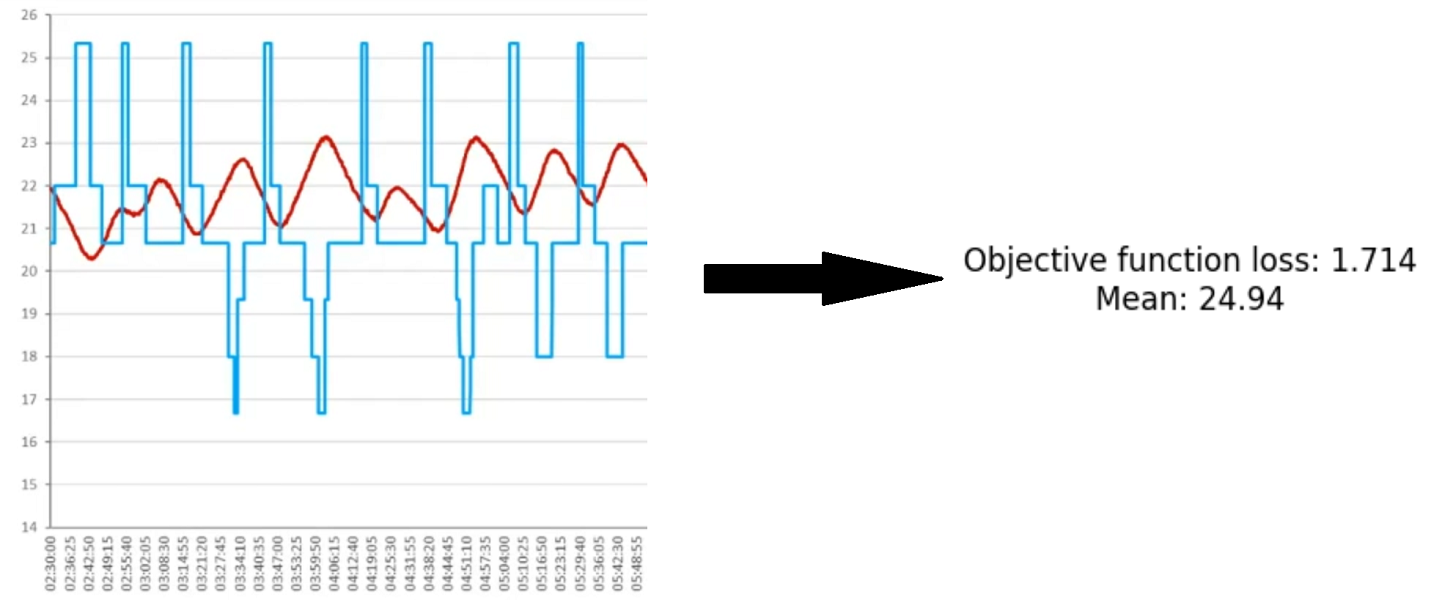
\includegraphics{objective_function}\\

Tak określony wzór daje nam dobrze zdefiniowany problem optymalizacyjny. Mianowicie im niższa wartość funkcji $F$ tym piec wydajniej pracuje.
\subsection{Model sieci neuronowej}
Maszynista stojący przed podjęciem decyzji o zmianie przepływu powietrza musi zadać sobie pytanie - jaką zmianę spowoduję? Kiedy on odpowiada sobie na nie na podstawie wiedzy i intuicji, my zaprzęgneliśmy algorytm sieci neuronowych badający tendencje i ukryte zależności danych. Nasz model potrafi podać jak zachowa się piec dla dowolnej akcji jaką można na nim wykonać. Rezultat ten otrzymaliśmy dzięki zastosowaniu rekurencyjnych sieci neuronowych (\textbf{LSTM})...

  
\subsection{Algorytm przeszukujący}
Gdy umiemy już przewidzieć jaką reakcję spowoduje dana akcja, możemy starać się odpowiedzieć na pytanie - jaki jest optymalny ciąg akcji na najbliższe kilka minut? A w szczególności na pytanie - jaką akcję powinno się podjąć w danym momencie? Zauważmy, że przeszukiwanie wszystkich możliwych akcji dla każdej sekundy z kolejnych paru minut, daje astronomicznej wielkości problem. Aby zmniejszyć przestrzeń poszukiwań i zarazm skupić się na rozwiązaniach sensowniejszych ograniczyliśmy możliwe ustawienia przepływu powietrza do dziewięciu opcji, natomiast dane zbierane co sekundę pogrupowaliśmy w sekcje 30-sekundowe. Chociaż liczba kombinacji możliwych akcji wciąż jest przerażająco wielka, to daje już pewne nadzieje na znalezienie ciągu sensownych decyzji. Aby tego dokonać zastosowaliśmy algorytm \textbf{Monte Carlo Tree Search} będący jednym z najbardziej zaawansowanych algorymów tej dziedziny informatyki. Jego własności:
\begin{itemize}
\item W przeszukiwaniu rozwiązań skupia się znacznie bardziej na tych dających lepsze rezultaty. Nie zapomina jednak całkiem o gorszych akcjach, ponieważ czasem ich drobna modyfikacja prowadzi do lepszych rezultatów, niż znalezione obecnie.
\item Jest algorytmem ANY-TIME, to znaczy, że skończy się kiedy my powiemy mu, aby się skończył. Innymi słowy im dłużej będzie działał, tym lepsze rezultaty osiągnie.
\item Daje możliwość zrównoleglenia, dzięki czamu stosując jego wersję zaimplementowaną na karcie graficznej uzyska się niesamowite przyspieszenie, a co za tym idzie poprawę efektywności.
\end{itemize}
Aby podkreślić skuteczność zastosowanego algorytmu można podać jego osiągi. Algorytm MCTS był podstawą do stworzenia systemu AlphaGo, który to jako pierwszy na świecie pokonał mistrza świata w chińskiej grze w Go.

\section{Podsumowanie}
Nasze podejście wykorzystuje jedne z najbardziej zaawansowanych i zoptymalizowanych algorytmów w danych dzidzinach, jednak nierozsądnym byłoby rezygnować z wiedzy, doświadczenia i intuicji osób pracujących z piecem na codzień. Te dwa podejścia do problemu można połączyć. Intuicje opisane odpowiednim językiem można przekazać komputerowi, a algorytmy które stosujemy są wprost przygotowane pod dołożenia kluczowego elementu jakim jest wiedza ekspertów. Dlatego najlepsze osiągi moglibyśmy uzyskać mierząc się z problemem wspólnie.

%\includegraphics{P3}

\end{document}
